\chapter{Persistierung} % (fold)
\label{cha:persistierung}

In den vorangegangen drei Kapiteln wurde die Umsetzung des eigentlichen Werkzeugs beschrieben. Neben der Unterstützung des Modellierungsvorgangs ist aber auch die persistente Speicherung der erstellten Modelle zum Zwecke der Weiterverarbeitung ein hier zu beleuchtender Aspekt. Auf die Persistierung wirken vor allem zwei der in Kapitel XY identifzierten Anforderungen ein. Zum ersten ist die Nachvollziehbarkeit des Modellierungsvorganges sicherzustellen -- dies gilt nicht nur während des Vorgangs selbst, sondern auch danach. Dementsprechend ist sämtliche Information zu persistieren, die zur Wiederherstellung nicht nur des Modells selbst sondern auch der gesamten Modellierungshistorie notwendig ist. Zum zweiten hat die Forderung nach semantischer Offenheit bei der Modellierung auch unmittelbare Auswirkungen auf die Persistierung. Neben dem Modell selbst muss aufgrund dieser Anforderung auch die Bedeutung der verwendeten Modellierungselemente miterfasst und persistiert werden, so dass diese bei der Weiterverarbeitung der Modelle verwendet werden kann.

In diesem Kapitel werden nun aufgrund der eben genannten Forderungen technologische Ansätze identifiziert, beschrieben und schließlich hinsichtlich ihrer Eignung für den konkreten Einsatz beurteilt. Der ausgewählte Ansatz wird im darauf folgenden Abschnitt konzeptuell beschrieben. Die Abbildung der Modelle und der ebenfalls zu persistierenden zusätzlichen Information in ein geeignetes Datenmodell ist Gegenstand des darauf folgenden Abschnitts. Schließlich wird die konkrete technische Umsetzung der Persistierung dargelegt und die dazu notwendigen Software-Module im Detail beschrieben.
 
\section{Möglichkeiten der Persistenzsicherung} % (fold)
\label{sec:möglichkeiten_der_persistenzsicherung}

\begin{itemize}
	\item Serialisierung von Java-Objekten
	\item Relationale Datenbanken
	\item XML Topic Maps
\end{itemize}

% section möglichkeiten_der_persistenzsicherung (end)

\section{Topic Maps} % (fold)
\label{sec:topic_maps}

Topic Maps \citep{TMDM08} sind wie bereits in Abschnitt XY beschrieben ein Mittel zur Abbildung von semantischen Netzen. In Topic Maps können beliebige Daten strukutriert aufbereitet und zueinander in Beziehung gesetzt werden. Die Art der zu repräsentierenden Daten ist dabei irrelvant, eine Topic Map trifft keine Aussage über ein den repräsentierten Daten zugrundeliegendes Begriffsystem (sie ist „ontology-agnostic“ \citep{Vatant04}).

Historisch stammen Topic Maps aus dem Bereich der technischen Repräsentation von Thesauri und Indizes \citep{Pepper00} \citep{Rath03}. Aus diesen Bereichen motivieren sich auch die Bausteine einer Topic Map, wenngleich der Verwendung durch diesen Ursprung nicht eingeschränkt wird. Die grundlegenden Elemente einer Topic Map sind „Topics“, „Associations“ und „Occurrences“ (siehe Abbildung \ref{fig:img_Persistenz_TMBasic}). 

\begin{figure}[htbp]
	\centering
		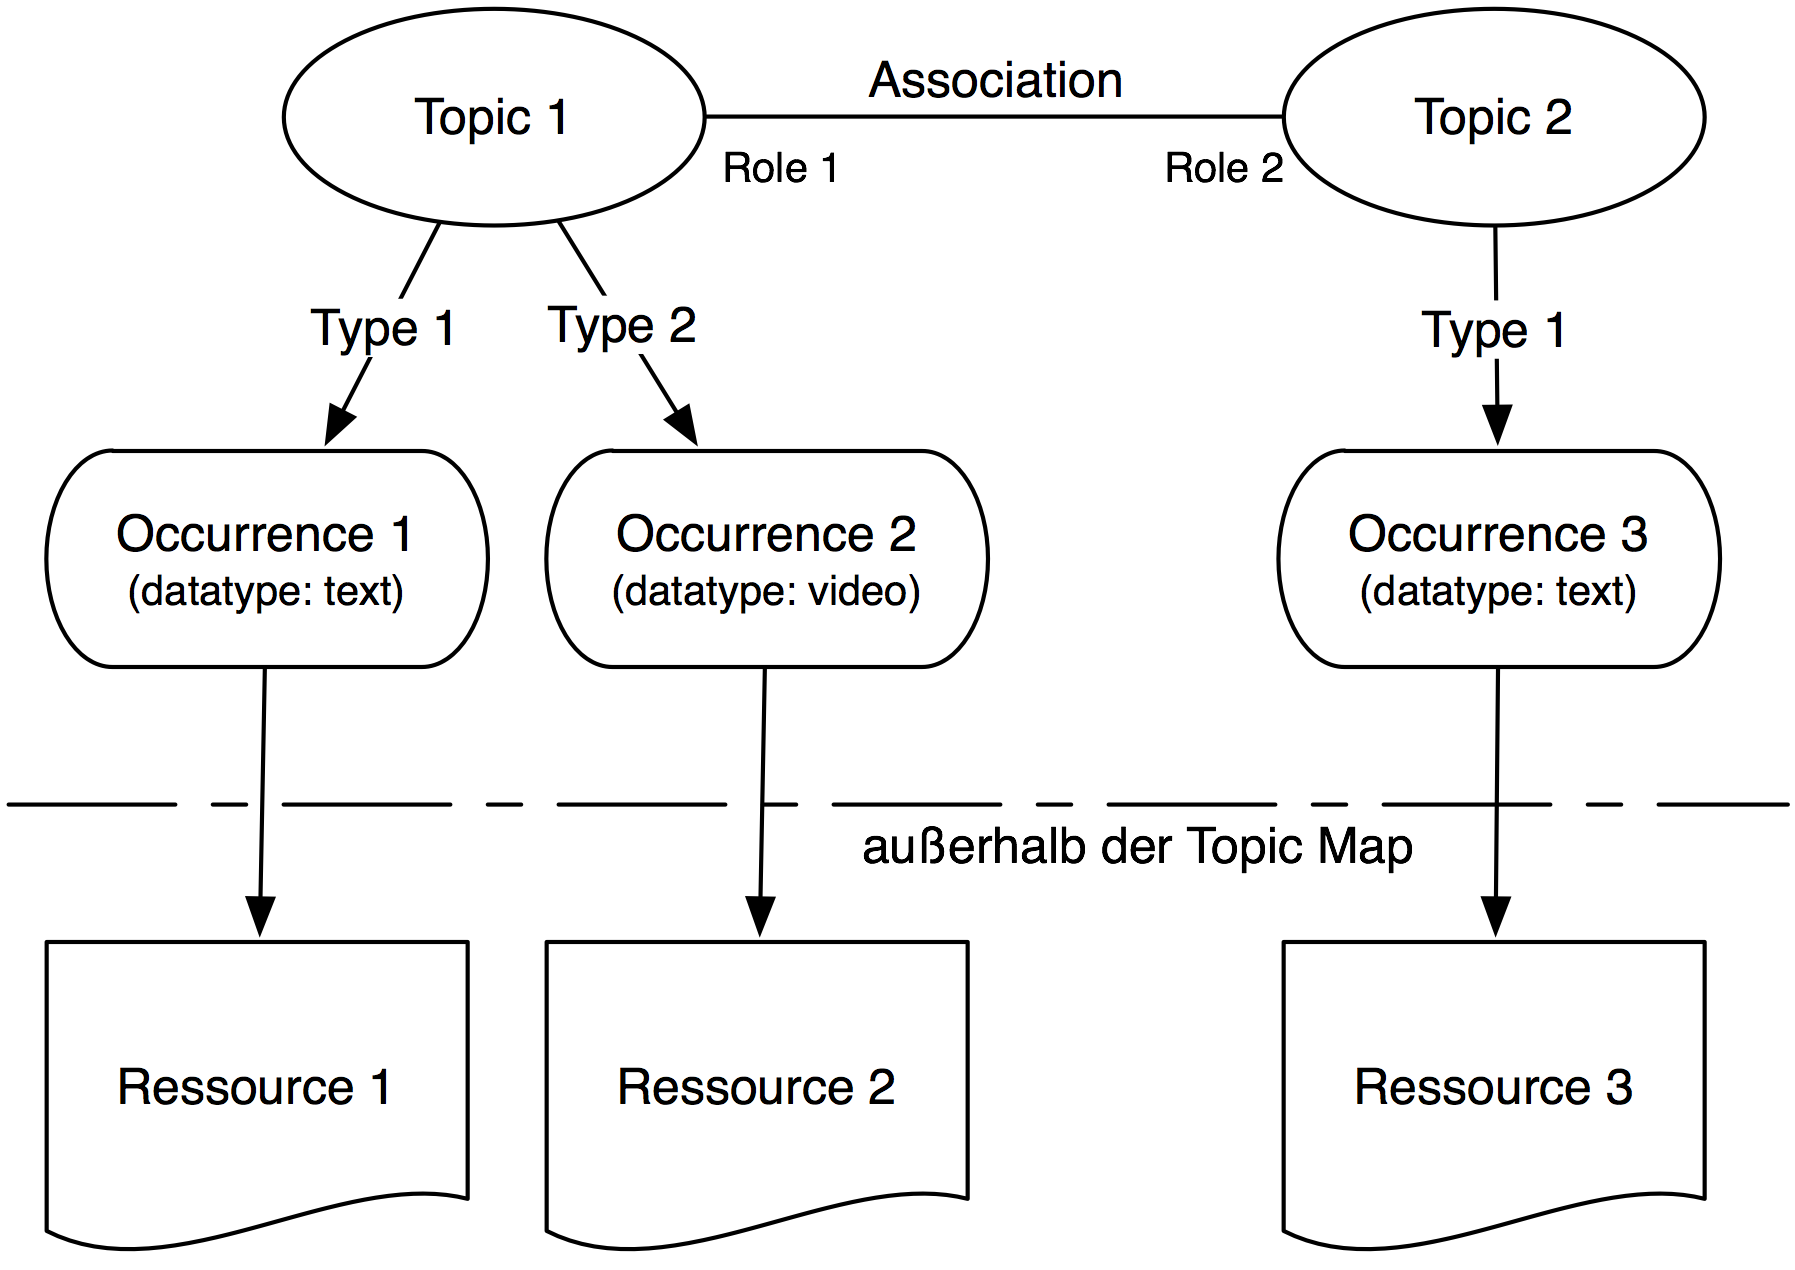
\includegraphics[width=10cm]{img/Persistenz/TMBasic.png}
	\caption{Grundlegende Elemente einer Topic Map}
	\label{fig:img_Persistenz_TMBasic}
\end{figure}

„Topics“ sind stellen Begriffe dar und bilden die Knoten des semantischen Netzes. Ein Topic kann beliebige Information darstellen, repräsentiert aber immer genau ein Phänomen der realen Welt (d.h. zu einem Topic muss es eine Entsprechung außerhalb der Topic Maps geben, die beobachtbar oder beschreibbar ist und auf die die modellierende Person Bezug nehmen will \footnote{„A subject can be anything whatsoever, regardless of whether it exists or has any other specific characteristics, about which anything whatsoever may be asserted by any means whatsoever. In particular, it is anything about which the creator of a topic map chooses to discourse.“ \citep[][S.8]{TMDM08}}). Eine Topic Map ist damit im Sinne von \citet{Stachowiak73} ein diagrammatisches Modell, das einen bestimmten, für den Modellersteller relevanten Ausschnitt der Realität abbildet.

"Associations" bilden die Beziehungen zwischen Topics ab und stellen damit die Kanten des semantischen Netzes dar. Eine Association verknüpft Topics semantisch miteinander und kann frei mit Bedeutung belegt werden. Die Art der Beziehungen ist also nicht festgelegt und wird wie die Bedeutung der Topics frei gewählt werden. Topics und Associations decken historisch den Bereich der Darstellung von Thesauri ab, in denen Begriffe definiert und zueinanden in Beziehung gesetzt werden. 

Der zweite historische Ursprung von Topic Maps, die Indizes, werden durch das Konstrukt der "Occurences" abgedeckt. Occurences ("Auftreten") sind Referenzen aus der Topic Map in die reale Welt. Sie setzen die Topics einer Topic Map in Bezug zu beliebiger referenzierbarer Information (z.B. Dokumente). Im Kontext der eben genannten Indizes, kann eine Topic Map als der mit Querverweisen versehene Index eines Buches verstanden werden, in dem durch die Angabe von Seitenzahlen auf den Text des Buches verwiesen wird. Diese Verweise durch Angabe der Seitenzahlen sind in diesem Zusammenhang die Occurrences.

Die Ansammlung von durch Associations verknüpften und mit Occurrences versehenen Topics bilden eine Topic Map. Darüber hinaus kann in Topic Maps jedoch noch weiterführende Information repräsentiert werden (siehe Abbildung \ref{fig:img_Persistenz_TMFull}), die Gegenstand der folgenden Abschnitte sein werden.

\begin{figure}[htbp]
	\centering
		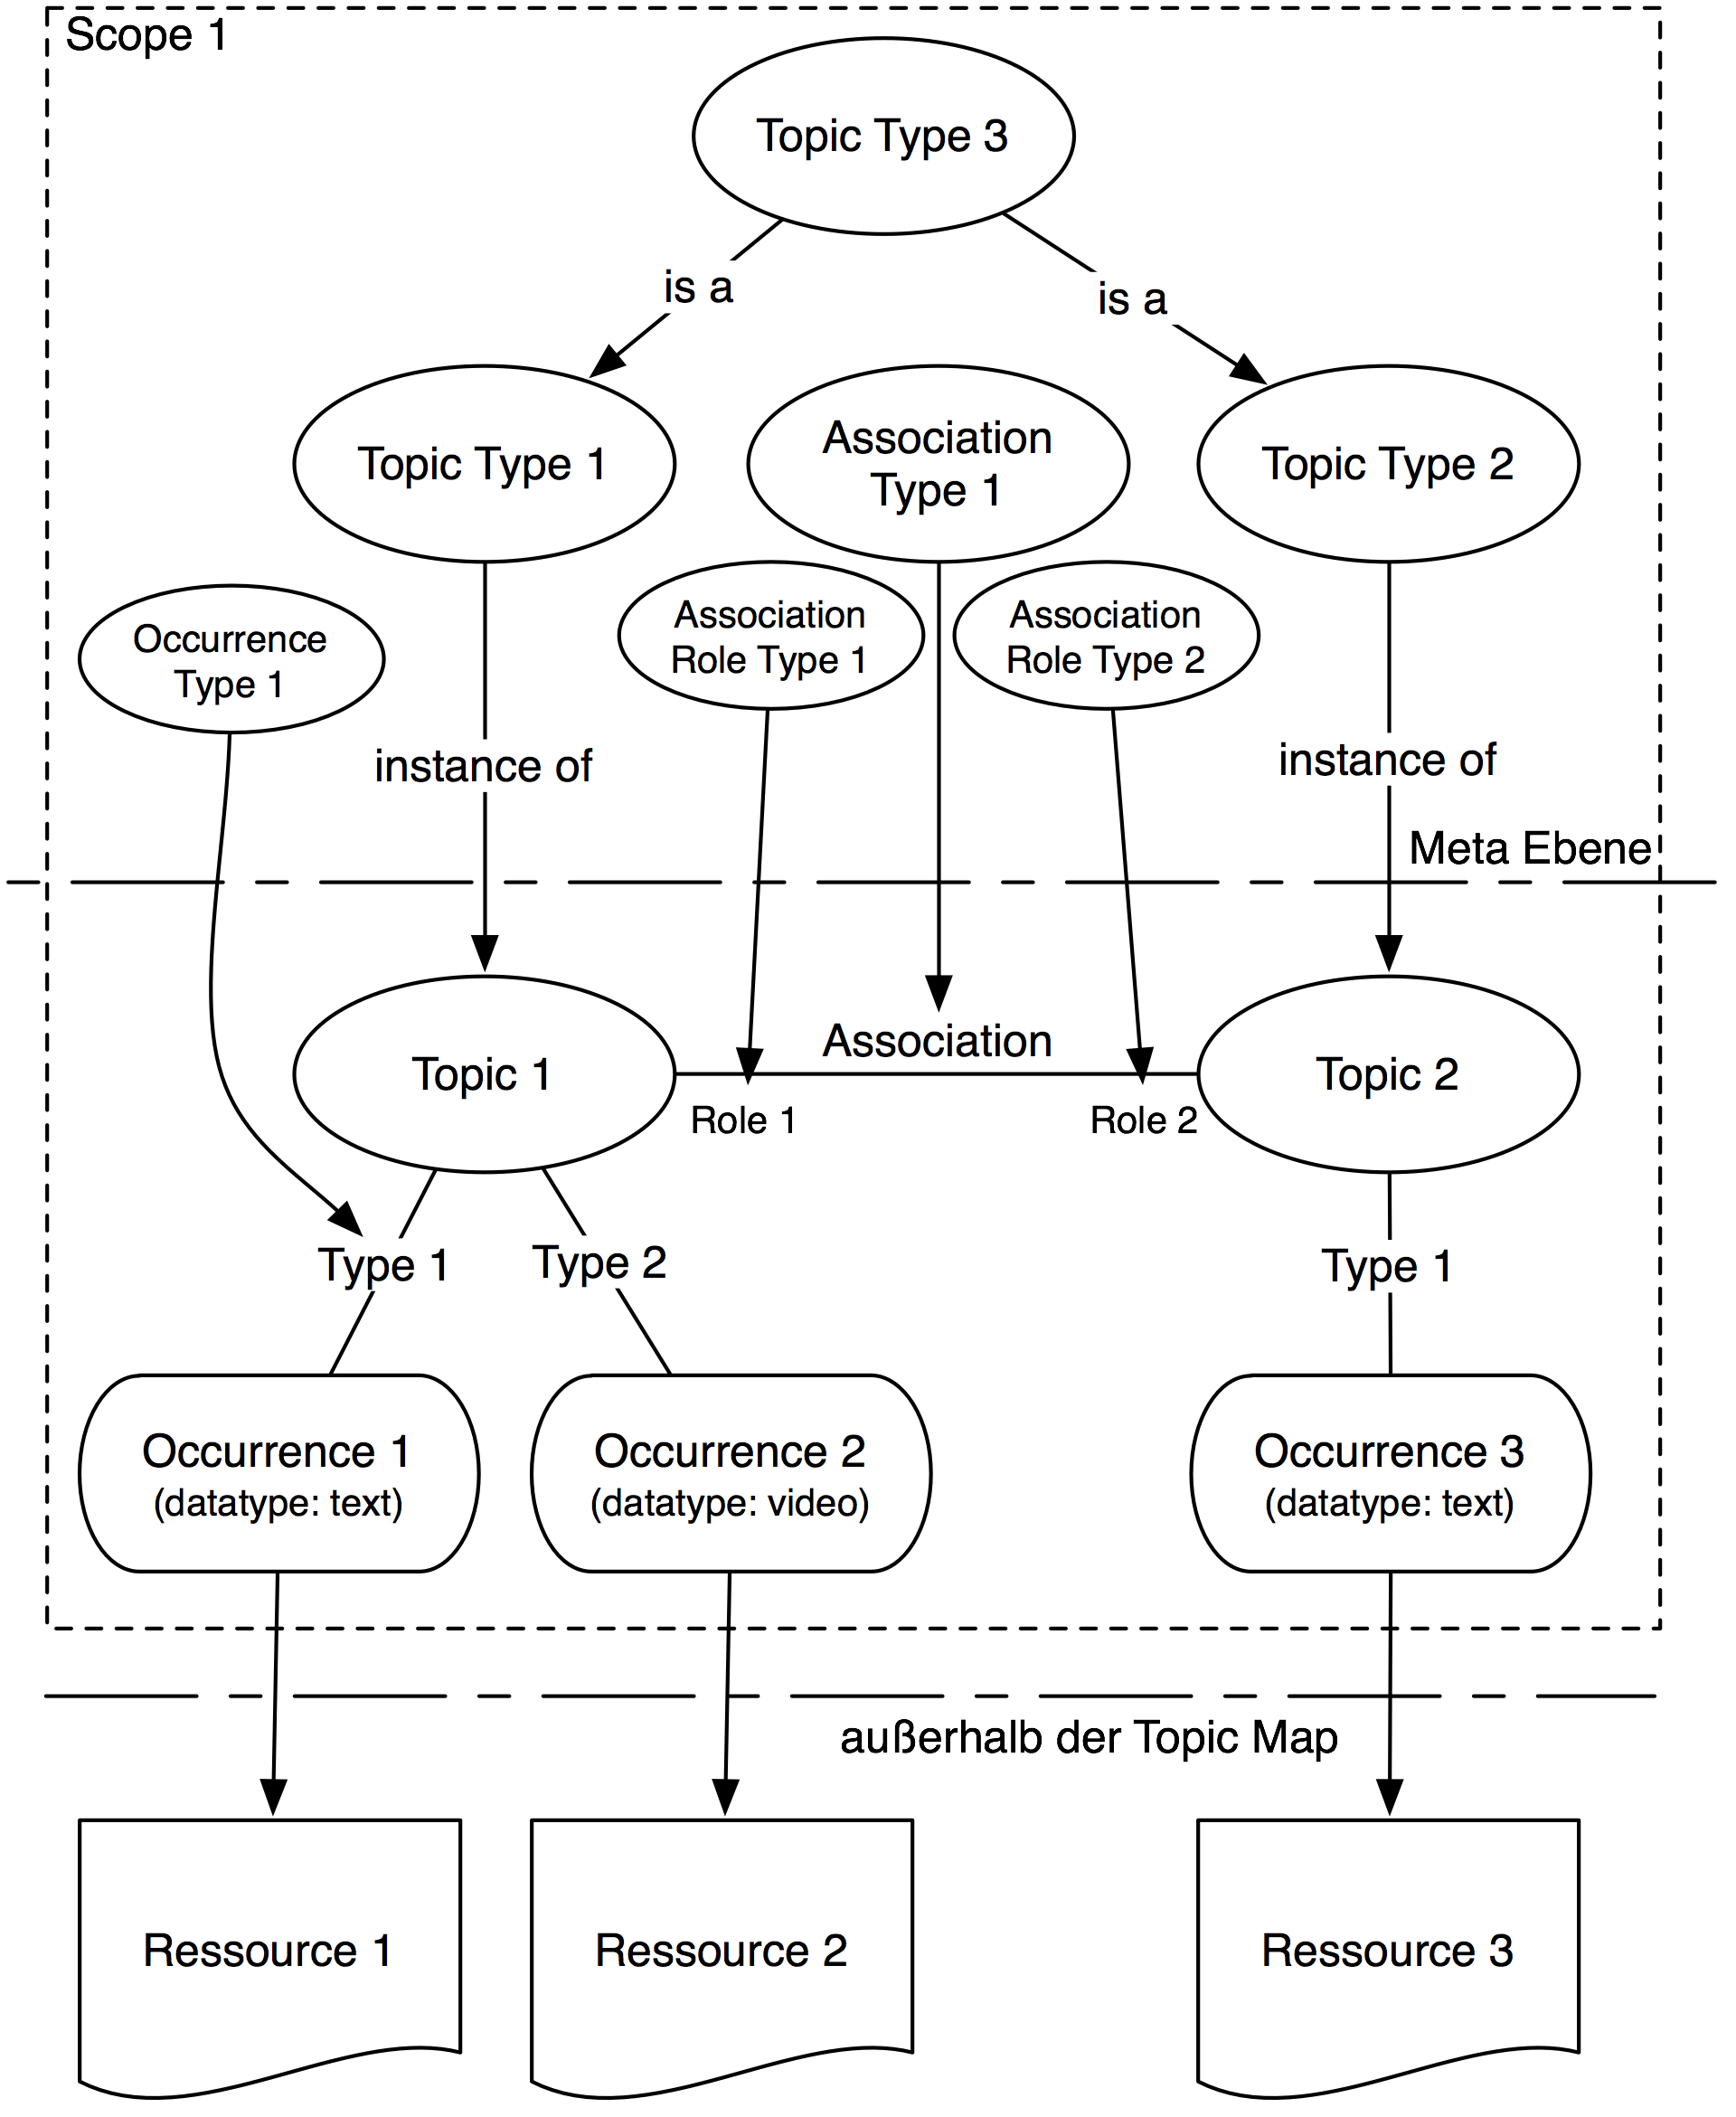
\includegraphics[width=10cm]{img/Persistenz/TMFull.png}
	\caption{Umfassende Darstellung der Elemente einer Topic Map}
	\label{fig:img_Persistenz_TMFull}
\end{figure}

\subsection{Topics, Subjects, Topic Names und Variants} % (fold)
\label{sub:topics_subjects_topic_names_und_variants}

Wie oben bereits beschrieben, repräsentiert ein Topic ein Phänomen der realen Welt in einer Topic Map. Dieses Phänomen der realen Welt, das durch das Topic repräsentiert wird, wird als „Subject“ bezeichnet. In einer Topic Map darf es zu einem Subject nur exakt ein Topic geben, umgekehrt kann ein Topic auch nicht mehrere Subjects repräsentieren, die Zuordnung zwischen Subject und Topic ist also eineindeutig (bijektiv). Im Topic wird dazu exakt ein „Subject Identifier“ registriert, der auf eine Informationsressource verweist, die das Subject für Menschen eindeutig identifizierbar macht (diese Ressource wird als „Subject Indicator“ bezeichnet). Zusätzlich kann ein „Subject Locator“ angegeben werden, der auf das tatsächlich in der realen Welt vorhandene Subject verweist. In Abgrenzung dazu kann es bei der anderen Brücke zwischen realer Welt und Topic Map, den Occurrences, für jeder Topic beliebig viele Zuordnungen geben. Eine Occurrence referenziert auch auf die reale Welt, zeigt aber dort nicht auf das Subject selbst, sondern auf ein dieses Subject beschreibendes Objekt in der realen Welt. Beispielhaft ist dazu in Abbildung \ref{fig:img_Persistenz_SubjectVsOccurrence} dieser Zusammenhang anhand des Topics „Tasse“ dargestellt. Ein anderes Beispiel ist ein Topic „London“, das als Subject die reale Stadt London repräsentiert und dem eine Occurrence zugeordnet werden könnte, die auf eine Landkarte (als in der Realität vorhandene Beschreibung der realen Stadt London) referenziert.

\begin{figure}[htbp]
	\centering
		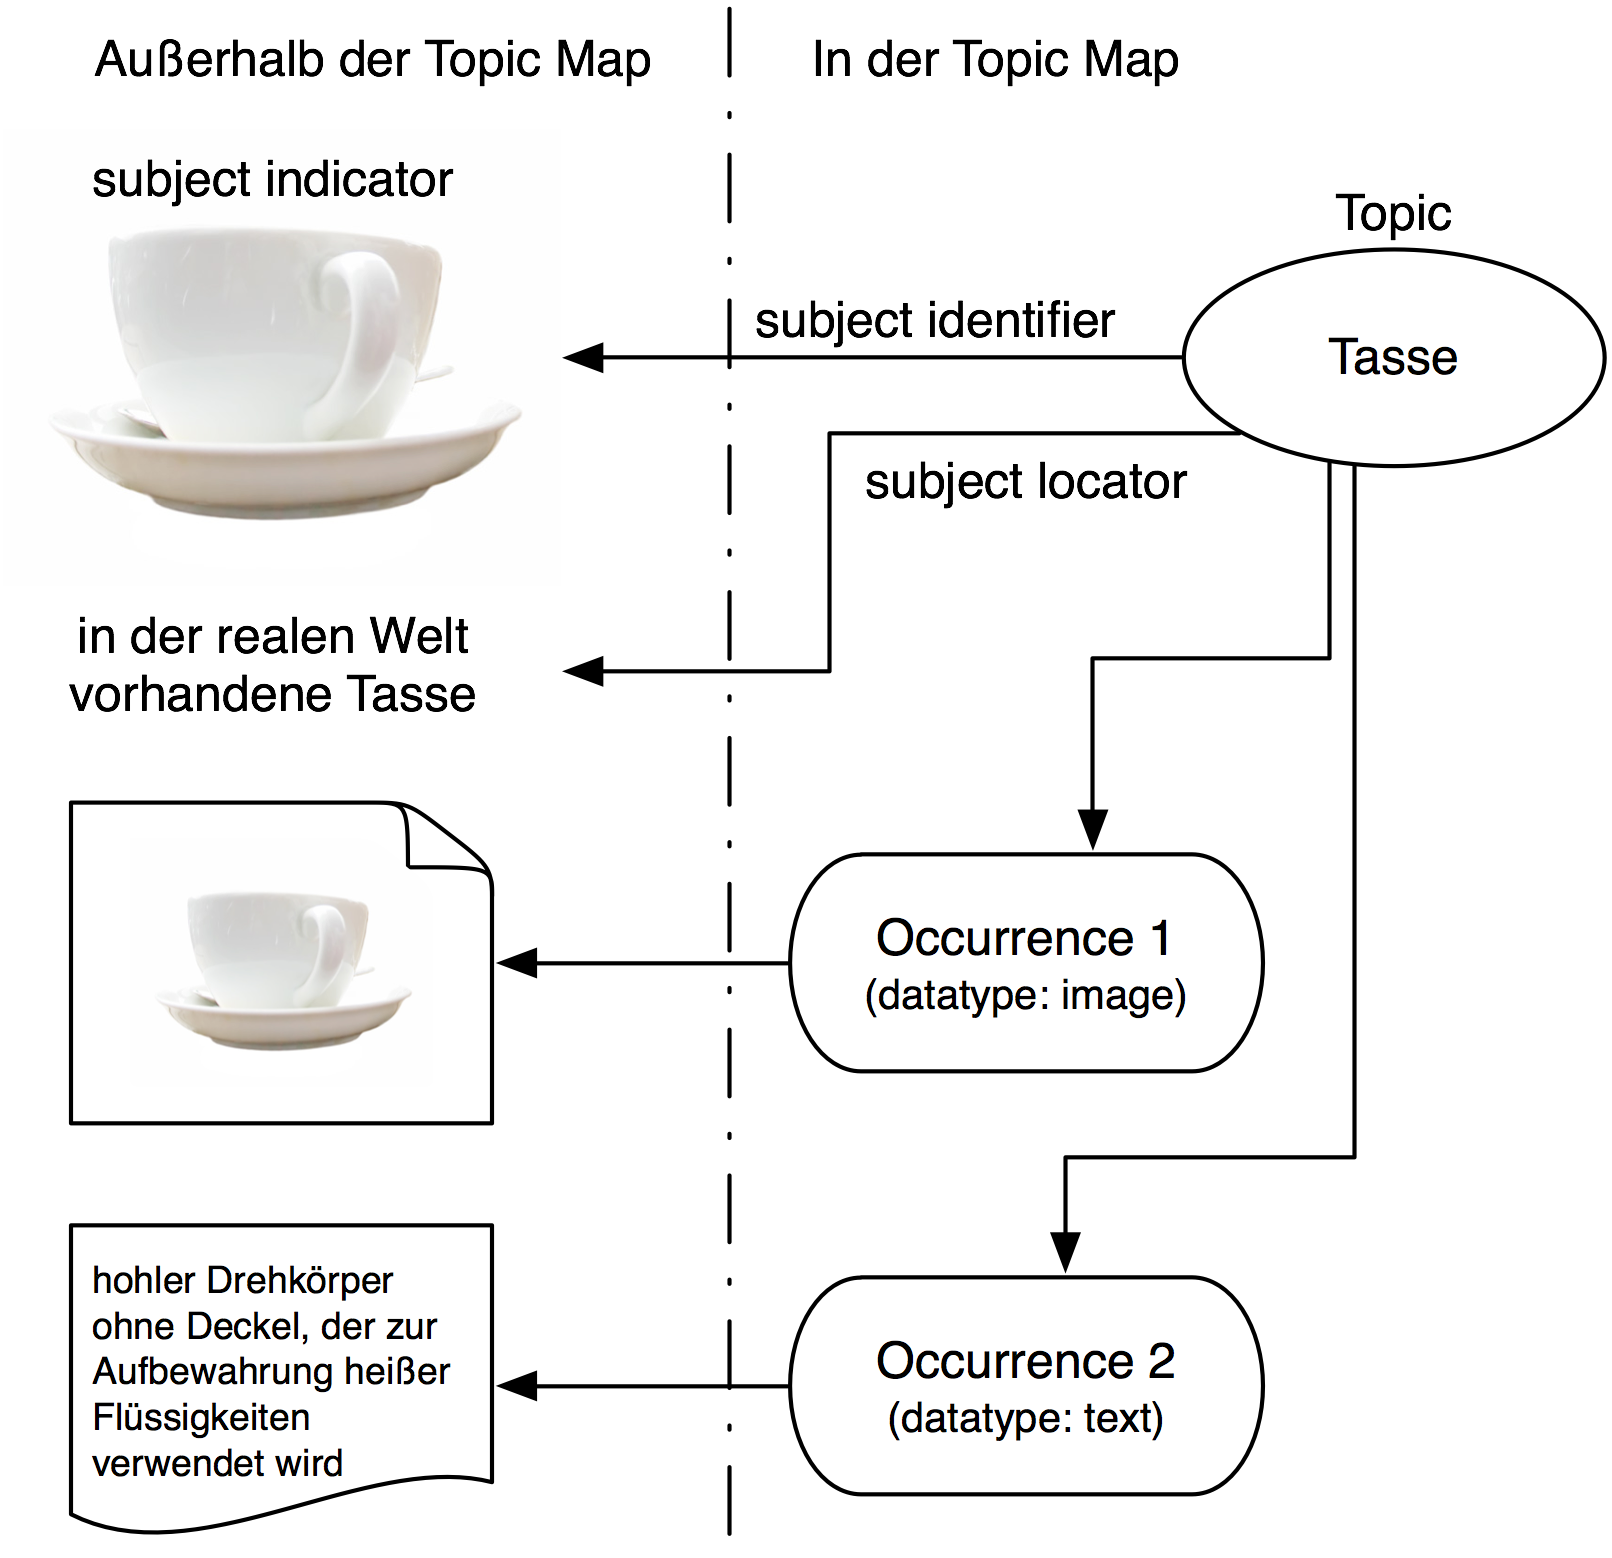
\includegraphics[width=10cm]{img/Persistenz/SubjectVsOccurrence.png}
	\caption{Abgrenzung zwischen Subject und Occurrence in Topic Maps}
	\label{fig:img_Persistenz_SubjectVsOccurrence}
\end{figure}

Bislang wurde vereinfacht ein Topic immer mit einem direkt zugeordneten Namen dargestellt. In einer Topic Map besitzt ein Topic jedoch keinen eindeutigen Namen. Es wird vielmehr durch seinen Subject Identifier eindeutig gekennzeichnet. Dieser ist jedoch nicht unbedingt für Menschen les- und/oder interpretierbar -- der Subject Identifier hat das Ziel, ein Subject für die Verarbeitung durch Software eindeutig zuordenbar zu machen. Für die Bezeichnung eines Topics in einer für Menschen interpretierbaren Form ist die Verwendung von „Topic Names“ vorgesehen (siehe Abbildung \ref{fig:img_Persistenz_TopicNaming}). Topic Names werden immer textuell angegeben und beschreiben das Subject, das durch das betreffende Topic referenziert wird. Durch einen Topic Name soll das Subject für Menschen erkennbar sein, wobei die Zuordnung nicht notwendigerweise eindeutig sein muss (Beispiel: der Topic Name „Jaguar“ kann ein Fahrzeug oder eine Großkatze bezeichnen und ist dementsprechend ein zulässiger Name für zwei unterschiedliche Topics). Einem Topic können beliebig viele Topic Names zugewiesen werden -- es ist so zum Beispiel möglich, eine mehrsprachige Topic Map zu realisieren, in der zu jedem Topic Topic Names in unterschiedlichen Sprachen angegeben werden. 

\begin{figure}[htbp]
	\centering
		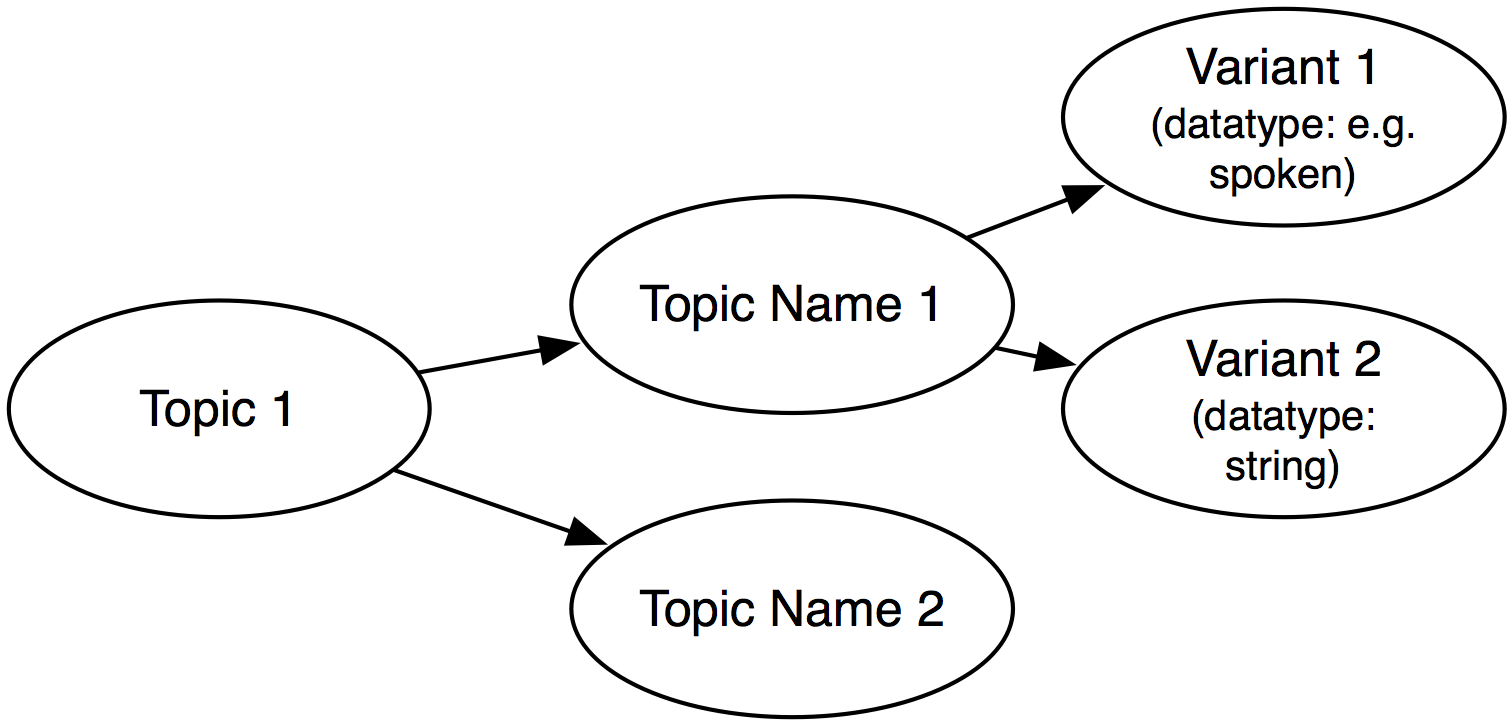
\includegraphics[width=10cm]{img/Persistenz/TopicNaming.png}
	\caption{Benennung von Topics}
	\label{fig:img_Persistenz_TopicNaming}
\end{figure}

Als weitere Detaillierungsstufe können zu jedem Topic Name „Variants“ angegeben werden. Wie durch den Namen angedeutet, handelt es sich dabei um Varianten eines Topic Names, die in bestimmten Zusammenhängen oder für gewisse Anwendungszwecke besser geeignet sein können als der eigentlich Topic Name. Ein Beispiel für eine mögliche Variante ist die Angabe einer gesprochenen Version des Topic Names. Ein weiteres Anwendungsgebiet für Varianten ist die im Standard explizit vorgesehene Angabe eines „Sort Name“ \citep[][S. 18]{TMDM08}, der es erlauben soll, Topic Maps in eine durch diesen Namen vorgegebene Ordnung bringen zu können. Varianten werden durch die Angabe eines dezidiert dafür gewidmeten Topics in deren Scope (siehe Abschnitt \ref{sub:scopes}) als Sort Names gekennzeichnet.

% subsection topics_subjects_topic_names_und_variants (end)

\subsection{Associations und Roles} % (fold)
\label{sub:associations_und_roles}

"Associations" stellen Verbindungen zwischen den einzelnen Topics einer Topic Map her. Associations haben beliebig viele Endpunkte, mindestens jedoch einen (sind also nicht von vorneherein immer binär sondern können auch unär sein oder mehr als zwei Topics verknüpfen). Eine Associations enthält wie ein Topic nicht unmittelbar einen für Menschen lesbaren Namen. Diese wird durch ein Topic festgelegt, das die Kategorie festlegt, der die Association zuzuordnen sind (siehe Abschnitt \ref{sub:metamodellierung_in_topic_maps}). Diesem Topic kann wiederum mindestens ein Topic Name zugeordnet werden, welcher letzendlich die Benennung der Association festlegt.

Associations werden jedoch nicht direkt mit Topics verknüpft. Um ausdrucksstärkere Verknüpfungen realisieren zu können, agieren "Roles" als Verknüpfung zwischen Association und den betreffenden Topics. Roles legen die "Rolle" -- also die Bedeutung -- eines Topics in exakt der betrachteten Association fest. Diese Bedeutung kann generisch sein und zum Beispiel dazu verwendet werden, die per se ungerichteten Associations unabhängig von ihrer konkreten Bedeutung mit einer Richtung zu versehen (zum Beispiel durch die Zuordnung von Roles "Anfang" und "Ende") aber auch um die Beziehung semantisch anzureichern (zum Beispiel durch die Zuordnung von Roles "Veranwortlicher", "Ausführender" und "Prozessschritt" in einer Association "durchzuführen"). Die Anzahl der in einer Association referenzierten Roles gibt damit auch die Kardinalität der Association (also die Anzahl ihrer Endpunkte) an. Aus den konkreten Roles wird dann auf die Topics verwiesen, die diese Roles einnehmen bzw. "spielen" (tatsächlich heißt die betreffende Eigenschaft einer Role "player"). Genau wie Associations werden Roles nicht direkt benannts sondern über ein Topic, das ihre Kategorie bestimmt, mit einer Benennung versehen (Detail wiederum in Abschnitt \ref{sub:metamodellierung_in_topic_maps}).

% subsection associations_und_roles (end)

\subsection{Occurrences und Datatypes} % (fold)
\label{sub:occurrences_und_datatypes}

Wie zu Beginn dieses Abschnitts bereits beschrieben und in den Erläuterungen zur Thematik der Subjects (siehe Abschnitt \ref{sub:topics_subjects_topic_names_und_variants}) angedeutet, bilden "Occurrences" die Brücke aus der Topic Map in die reale Welt, indem sie auf Ressourcen referenzieren, die in einem beliebigen Zusammenhang mit den jeweiligen Topic stehen. Ein Topic kann beliebig viele Occurrences haben. Anders als bei Associations existieren für Occurrences keine Roles (was auch nur bedingt sinnvoll wäre, da jede Occurrence nur zu exakt einem Topic gehören kann). Die Bedeutung der Occurrence für das Topic kann wie bei Associations über die Kategorie der Occurrence festgelegt werden, die wiederum durch ein separates Topic repräsentiert wird (siehe dazu auch Abschnitt \ref{sub:metamodellierung_in_topic_maps}). Beispielsweise kann eine Occurrence zur Kategorie "Karte" gehören und so angeben, dass die so klassifizierte Occurrence zum Topic "London" auf eine Karte des Stadtgebiets verweist.

Zusätzlich zu der Kategorie wird in einer Occurrence auch der Datentyp der Information angegeben, in dem die referenzierte Information vorliegt. Dabei können beliebige URI (Uniform Resource Identifiers\footnote{wie in RFC 3986 definiert und unter http://www.ietf.org/rfc/rfc3986.txt abzurufen}) verwendet werden. Da URIs beliebigen Inhalt haben können, wäre es in obigen Beispiel möglich durch den Datentyp einer Occurrence festzulegen, ob es sich bei der Karte um eine Rastergrafik oder eine Vektorgrafik handelt und so Information über deren möglich Einsatzgebiete zu einzubetten.

% subsection occurrences_und_datatypes (end)

\subsection{Metamodellierung in Topic Maps} % (fold)
\label{sub:metamodellierung_in_topic_maps}

Wie oben bereits mehrmals angedeutet kann in einer Topic Map neben den eigentlichen zu repräsentierenden Informationen (Topics, Associations, Roles und Occurrences) auch Information über die Topic Map selbst eingebettet werden (neben dem Model also auch das Meta-Modell abgebildet werden kann). Die Information umfasst Angaben über die in der jeweiligen Topic Map existierenen Kategorien von Topics, Topic Names, Associations, Roles und Occurrences. Hinsichlich der Repräsentation dieser Information sind zwei Ansätze zu unterscheiden, von denen der erste bei Kategorieangaben von Topics zum Einsatz kommt, der andere bei Kategorieangaben jeder anderen Art von Information. Allen Kategorien ist gemein, dass sie selbst wiederum als Topics repräsentiert werden und auch als solche verwendet werden können. Es ist also möglich, zu einem Topic, das als Kategorie verwendet wird, selbst wiederum eine Kategorie anzugeben, wodurch die Einführung beliebig vieler Meta-Ebenen möglich ist. Außerdem können als Kategorien verwendete Topics ebenfalls wieder mit Associations verknüpft und mit Occurrences versehen werden. Hinsichtlich der Nomenklatur ist noch darauf hinzuweisen, dass Kategorien im Allgemeinen als "Types" bezeichnet werden, man also von "Topic Types", "Topic Name Types", "Association Types", "Role Types" und "Occurrence Types" spricht.

\subsubsection{Topic Types}

Topic Types werden in einer Topic Map durch ein spezielle, im Standard festgelegte Association definiert. Soll einem Topic ein Type zugewiesen werden, muss eine Association der Kategorie "type-instance" eingefügt werden, bei der das Topic selbst die Role "instance" einnimmt und dem Topic, das die Kategorie repräsentiert, die Role "type" zugewiesen wird. Diese Beziehung entspricht einer Konkretisierung eine (abstakten) Kategorie oder Klasse von Topics auf eine bestimmte Instanz, die die Merkmale dieser Klasse trägt. In Abbildung \ref{fig:img_Persistenz_MetaModelExample} besteht eine type-instance-Beziehung (dort als "instance-of" bezeichnet) zwischen der Kategorie "VW Golf" und der konkreten Instanz "SR-174 AU" (also einem Topic, bei dem das amtliche Kennzeichen als Topic Name verwendet wurde). "VW Golf" fungiert hier also als Topic Type, wobei es selbst ein Topic ist, das sich durch nichts als die eingenomme "type"-Rolle von einem anderen Topic unterscheidet und dementsprechend behandelt werden kann.

Einem Topic können beliebig viele Topic Types zugewiesen werden, indem es in mehr als einer Association die Role "instance" einnimmt. Es wird so als mehreren Kategorien zugehörig gekennzeichnet. Umgekehrt kann ein Topic Type mehr als einem Topic zugewiesen werden, indem das betreffende den Topic Type repräsentierende Topic die Role "type" mehrfach einnimmt.

\begin{figure}[htbp]
	\centering
		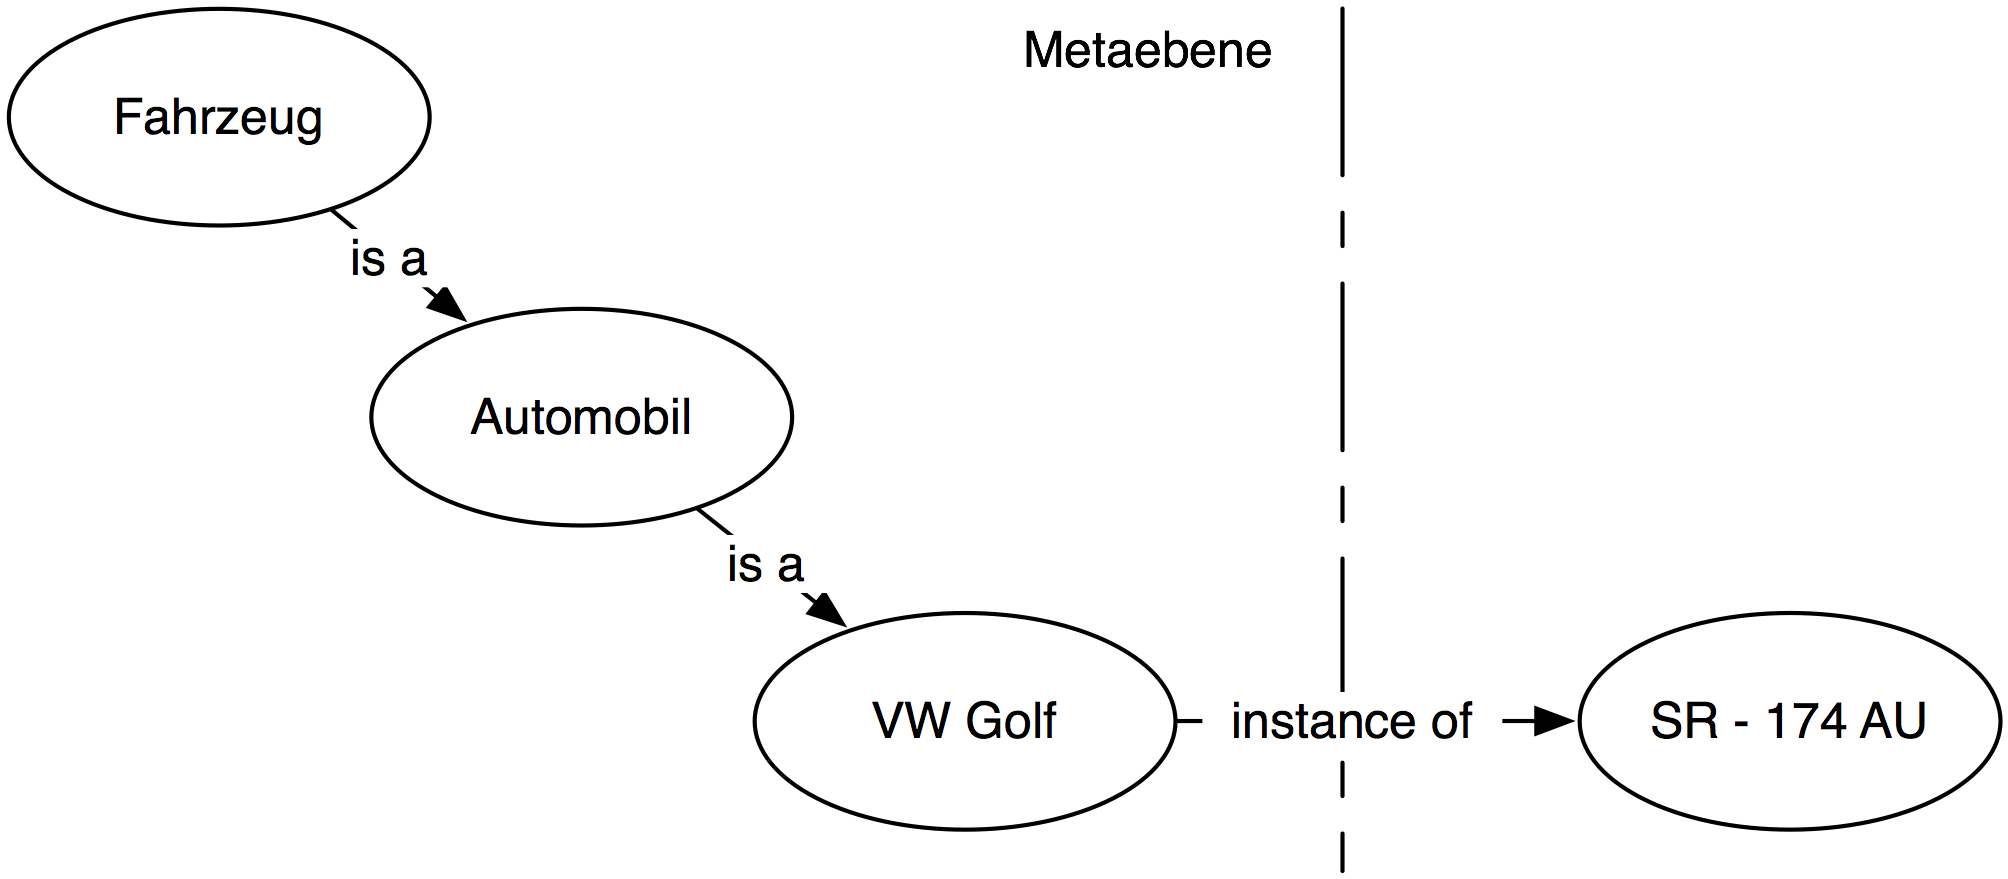
\includegraphics[width=10cm]{img/Persistenz/MetaModelExample.png}
	\caption{Beziehungen in der Metamodellbildung in Topic Maps}
	\label{fig:img_Persistenz_MetaModelExample}
\end{figure}

Auch ist es möglich, Hierarchien von Types zu bilden, in dem einem Topic, das als Topic Type fungiert, selbst wieder ein Topic Type zugewiesen wird. Dieses Konstrukt ist jedoch mit Vorsicht zu gebrauchen, da zur Abbildung der Struktur einer Domäne ein semantisch ähnliches, bei näherer Betrachtung aber eine unterschiedliche Bedeutung tragendes Konstrukt zum Einsatz kommt. Grundsätzlich muss unterschieden werden, ob ein Topic eine konkrete Instanz eines anderen ist oder lediglich eine Spezialisierung darstellt. Im ersteren Fall kommt eine "type-instance" zum Einsatz, das übergeordnete Topic befindet sich semantisch auf eine anderen, abstrakteren Ebene und stellt eine Kategorie (also einen Topic Type) dar. Im Falle einer Spezialisierung kommt eine "supertype-subtype"-Association zum Einsatz, deren Rollen "supertype" vom übergeordneten, allgemeineren bzw. "subtype" vom untergeordneten, spezielleren Topic eingenommen wird. Hier befinden sich beide Topics semantisch auf einer Ebene, keines ist abstrakter als das andere. Der Unterschied liegt vielmehr in der mehr oder weniger konkreten Festlegung der durch die Topics repräsentierten Subjects. So ist wie in Abbildung \ref{fig:img_Persistenz_MetaModelExample} dargestellt das Topic "VW Golf" ein Subtype des Topics "Automobil" welches wiederum ein Subtype des Topics "Fahrzeug" ist. Hier ist erkennbar, dass "Automobil" insofern eine Spezialisierung von "Fahrzeug" ist, als dass es im Allgemeinen motorisiert ist und vier Räder besitzt. "VW Golf" ist wiederum eine Spezialisierung von Fahrzeug, die hinsichtlich der Form der Karosserie, der Anzahl der Türen und anderen Merkmalen mehr spezialisiert. Zwischen keinem der Topics findet jedoch eine Konkretisierung in dem Sinne statt, als dass auf der untergeordneten Seite von einem konkreten, real existierenden Fahrzeug die Rede wäre -- dazu ist die "type-instance"-Beziehung zu verwenden. Die "subtype-supertype"-Beziehung ist transitiv, d.h. dass ein "VW Golf" nicht nur ein "Automobil" ist, sondern auch ein "Fahrzeug". Für "type-instance"-Beziehungen ist diese Eigenschaft nicht gegeben. 

\subsubsection{Andere Types}

Bei allen anderen Types (konkret also Topic Name Types, Association Types, Role Types und Occurrence Types) wird die Kategorie nicht durch eine separate Association abgebildet sondern durch eine im jeweiligen Informationselement enthaltene Referenz auf ein Topic, das als Type fungiert. Die Darstellung der Kategorie-Information ist damit nicht so explizit wie bei Topic Types, wo sich direkt in der Repräsentation der eigentlichen Nutzinformation niederschlägt. Auch semantisch ist sind die hier behandelten Types gegenüber Topic Types insofern eingeschränkt, als das jedem Element exakt ein Type zugeordnet sein muss (der Type kann also nicht leer sein, auch können nicht mehrere Types zugeordnet werden). Wie oben bereits erwähnt sind Topic Types hier flexibler, einem Topic können beliebig viele oder auch keine Topic Types zugeordnet werden. Dies ist aber nur vordergründig eine Einschränkung. Topics dürfen wie oben beschrieben für jedes Subjekt nur einmal existieren. Hat aber ein Subject und damit ein Topic in unterschiedlichen Domänen unterschiedliche Bedeutungen, muss dies über mehrere Topic Types (in Verbindung mit Scopes, siehe Abschnitt \ref{sub:scopes}) abgebildet werden. Alle anderen Informationskategorien in der Topic Map unterliegen nicht dieser Eineindeutigkeitsregel und können bzw. müssen, sollten sie unterschiedlichen Kategorien zuzuordnen sein, auch mehrfach vorhanden sein. Eine Assoziation, die einen anderen Namen trägt (also einer anderen Kategorie angehört) ist beispielsweise nicht identisch mit der ursprünglichen Assoziation, deren Name ebenfalls bereits durch die Zuordnung zu einer Kategorie festgelegt wurde. 

% subsection metamodellierung_in_topic_maps (end)

\subsection{Statements und Scopes} % (fold)
\label{sub:scopes}

Topic Maps bieten die Möglichkeit, Gültigkeitsbereiche für die in ihnen abgebildeten Informationen zu spezifizieren. Ein Gültigkeitsbereich definiert, in welchem Kontext eine Information gültig ist. Außerhalb dieses Kontext kann über die Gültigkeit keine Aussage getroffen werden. Der Gültigkeitsbereich wird als "Scope" bezeichnet. Ein Scope kann für jedes "Statement" in der Topic Map gesetzt werden. Statements sind alle "Aussagen" über Topics, die in der Topic Map abgebildet werden, nicht aber Topics selbst. Als Statement werden Topic Names, Associations und Occurrences betrachtet. Roles und Variants besitzen keinen Scope, da sie keine direkte Aussage über Topics treffen, sondern nur im Zusammenhang mit Associations bzw. Topic Names existieren, deren Scope sich quasi auf sie vererbt.

Ein Scope für ein Statement wird durch die Angabe eines oder mehrerer Topics festgelegt. Wird kein Topic angegeben, so gilt der "unconstrainted scope", das Statement ist unbeschränkt gültig. Topics zur Abbildung von Scopes können explizit angelegt werden (z.B. Topics "Deutsch" und "Englisch", die Sprach-Scopes ermöglichen, Topics "Tierwelt" und "Transportwesen" zur Domänenabgrenzung), es ist jedoch grundsätzlich auch möglich, die Gesamtheit der Topics einer Domäne zur Definition eines betreffenden Scopes heranzuziehen (also alle in der Topic Map vorhandenen Topics, die Tiere repräsentieren, als Scope zu verwenden, um den Gültigkeitsbereich "Tierwelt" abzubilden). Obwohl der Topic Map Standard hier explizit offen bleibt, erscheint jedoch erstere Variante hinsichtlich der Verwaltbarkeit aber auch der semantischen Vollständigkeit wegen als ratsamer (das Konzept "Tierwelt" käme ansonsten z.B. nicht notwendigerweise vor, sondern wäre nur implzit vorhanden, was eine Auswertung schwierig macht).

-- Abbildung Jaguar, Räder, Punkte jeweils mit Beziehung "hat" - Scope Tierwelt und Automobile ... --

Wird mehr als ein Topic angegeben, so bilden alle Topics gemeinsam den Kontext, indem das Statement gültig ist. Bei der Auswertung des Gültigkeitsbereichs müssen also alle angegebenen Topics zutreffen, damit ein Statement gültig ist. Ein Statement dessen Scope die Topics "Tierwelt" und "Deutsch" enthält, ist also nur gültig, wenn beide Topics zutreffen (also z.B. zur Filterung ausgewählt wurden). Die gültigen Statements sind also die Schnittmenge jener der Statements, die im Scope "Tierwelt" und im Scope "Deutsch" gültig sind. Die Angabe eines Scopes zu einem Statement, das in beiden Scopes (unabhängig voneinander gesehen) gültig sein soll, ist nicht direkt möglich. In diesem Fall muss das Statement zweimal jeweils unter Angabe eines der beiden Scopes eingefügt werden.

% subsection scopes (end)

\subsection{Weiterführende Konzepte} % (fold)
\label{sub:tm_weiterführend}

\subsubsection{Reification} % (fold)
\label{ssub:reification}

% subsubsection reification (end)

\subsubsection{Merging} % (fold)
\label{ssub:merging}

% subsubsection merging (end)
% subsection tm_weiterführend (end)

\subsection{Einschränkungen} % (fold)
\label{sub:einschränkungen}

Regeln und verbindliche Strukturvorgaben
Datenhaltung und Abfrage
% subsection einschränkungen (end)
% section topic_maps (end)

\section{Abbildung von Modellen auf Topic Maps} % (fold)
\label{sec:abbildung_von_modellen_auf_topic_maps}
-> DA Matthias
% section abbildung_von_modellen_auf_topic_maps (end)

\section{Technische Umsetzung der Persistierung von Modellen} % (fold)
\label{sec:technische_umsetzung_der_persistierung_von_modellen}
Topic Map Engine Persistence Layer
% section technische_umsetzung_der_persistierung_von_modellen (end)

\section{Zusammenfassung} % (fold)
\label{sec:persistierung_zusammenfassung}

% section persisitierung_zusammenfassung (end)
% chapter persistierung (end)
